\section{Distribution and Documentation}

The GEMC framework is documented on the GEMC website \cite{GEMC}. This includes the latest news and releases,
examples, procedure details, and documentation for all the available options.
The software is distributed in two ways: with docker \cite{jlabDocker}, or by downloading the source from the public git repository.

A docker container with the necessary libraries to run GEMC and the reconstruction software
is created in the Jefferson Lab hub repository.
The container is tagged, and every tag contains a set version of these libraries:

\begin{itemize}
	\item pythia-based event generators for various physics channels relevant to the CLAS12 analyses;
	\item GEMC with the CLAS12 geometry;
	\item the java reconstruction software \cite{recon-nim}.
\end{itemize}


The code git repository is \url{https://github.com/gemc/source}, which is a public repository.
The development contribution mechanism is illustrated in \F{github}: collaborators fork the repository
and make pull requests that are validated by the code author.
GEMC is released on a semi-annual cycle.

\begin{figure}
	\centering
	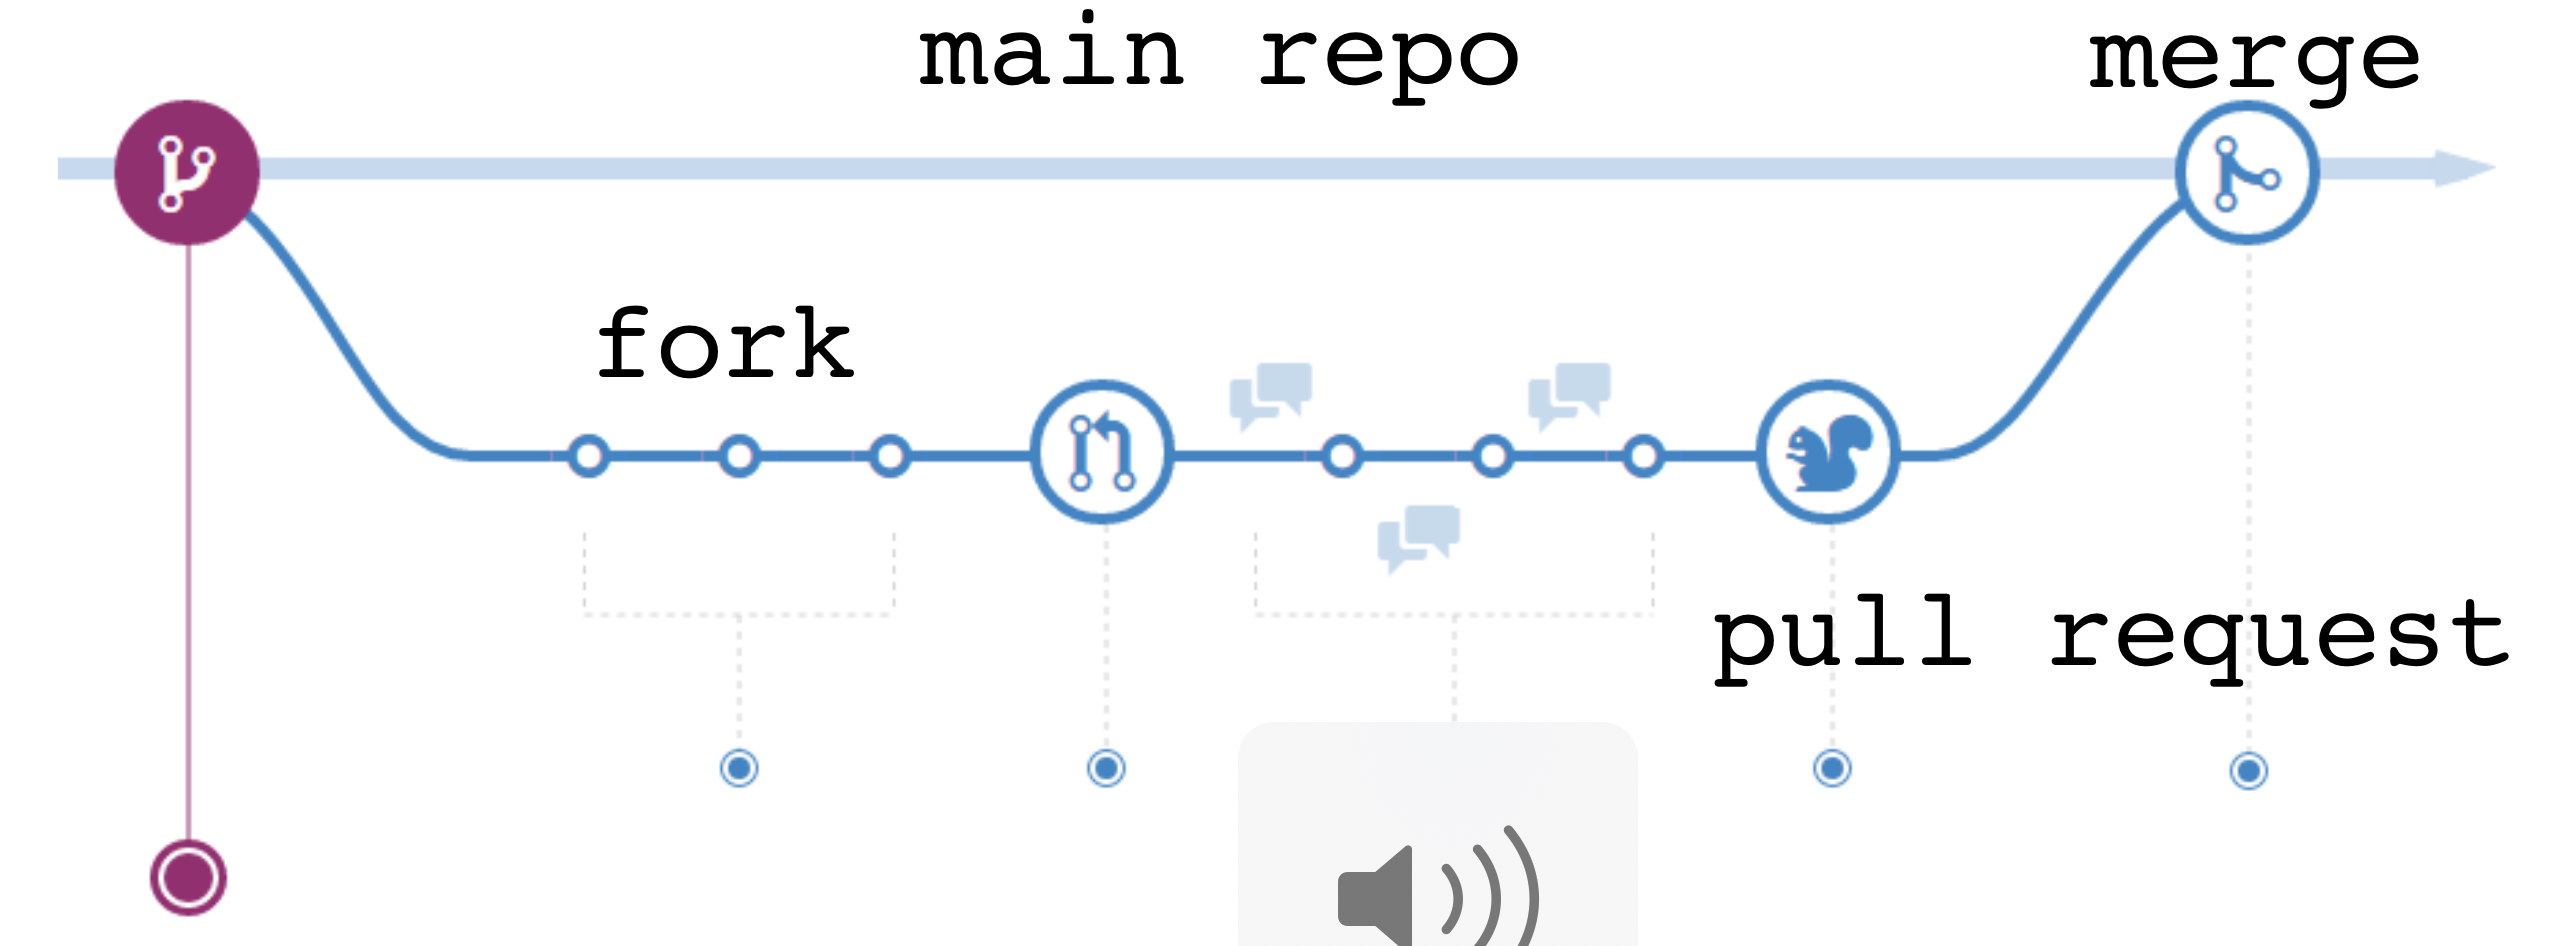
\includegraphics[width=0.99\columnwidth,keepaspectratio]{img/github.png}
	\caption{Typical workflow of contribution to the code. First, the main repository is forked and worked on. Then, during the fork code developments,
	         comments can be made on the various commits. Lastly, when the users make the pull request, the changes are validated and then merged
             to the master repository (or sent back with comments if there were problems).}
	\label{fig:github}
\end{figure}


The list of software packages included in the GEMC framework is:

\begin{itemize}
	\item clhep: Class Library for High Energy Physics \cite{clhep};
	\item xercesc: validating XML parser \cite{xercesc};
	\item Geant4: the libraries to simulate the passage of particles through matter \cite{geant4};
	\item qt: a C++ graphic library \cite{qt};
	\item evio: the CLAS12 data format \cite{evio};
	\item CCDB: the calibration database based on mysql \cite{ccdb}.
\end{itemize}

The main documentation is on the GEMC website \cite{GEMC}. It includes examples of how to create and run a custom geometry
and use various features like event generators, geometry factories, hit definitions, output, etc.

The CLAS12 development of both hit process routines and geometry is kept on the CLAS12 tags portal \cite{clas12Tags},
which also contains documentation on how to run with configurations corresponding to the various experiments, how to change the
beamline configuration, and how to switch between code and geometry releases.





